\chapter{Submission Tool for Students}
\label{Kapitel Aufruf}
The student interface can be opened under cis.technikum-wien.at/My CIS/Bachelor's and Master's Thesis Submission.

\section{Overview List of the Supervised Theses}
You can find all supervised Bachelor's and Master's theses in the overview list (see Fig. \ref{abgabetool_uebersicht_student}).

\begin {figure}
	\centering
	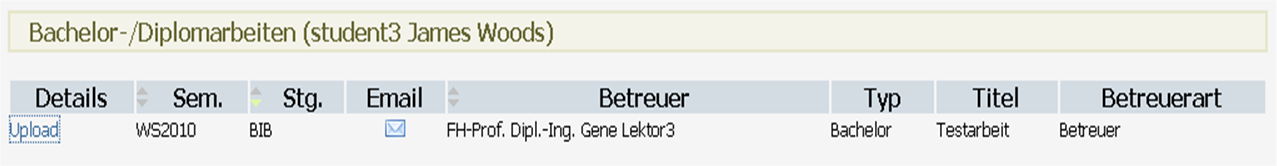
\includegraphics[width=1.0\textwidth]{abgabetool_uebersicht_student}
	\caption{Overview List of the Supervised Theses}
	\label{abgabetool_uebersicht_student}
\end {figure}

\subsection{Viewing the Deadline Overview}
The deadline details are displayed in the bottom portion of the page (see Fig. \ref{abgabetool_termine_student}) by clicking on \textit{Upload} in the first column of the overview list.

\subsection{Emailing the Supervisor}
By clicking the letter icon in the third column, the email client will open and fields for the recipient and sender addresses as well as the subject \textit{Bachelor's Thesis Supervision} or, \textit{Master's Thesis Supervision} will be automatically filled out.

\subsection{Opening the Instructions}
On the right side next to the heading \textit{Bachelor's/Master's Thesis Supervision} you will find a blue icon with a white i in the middle. Simply click on this symbol to open the instructions as a pdf file.

\section{Deadline Overview}

\begin {figure}
	\centering
	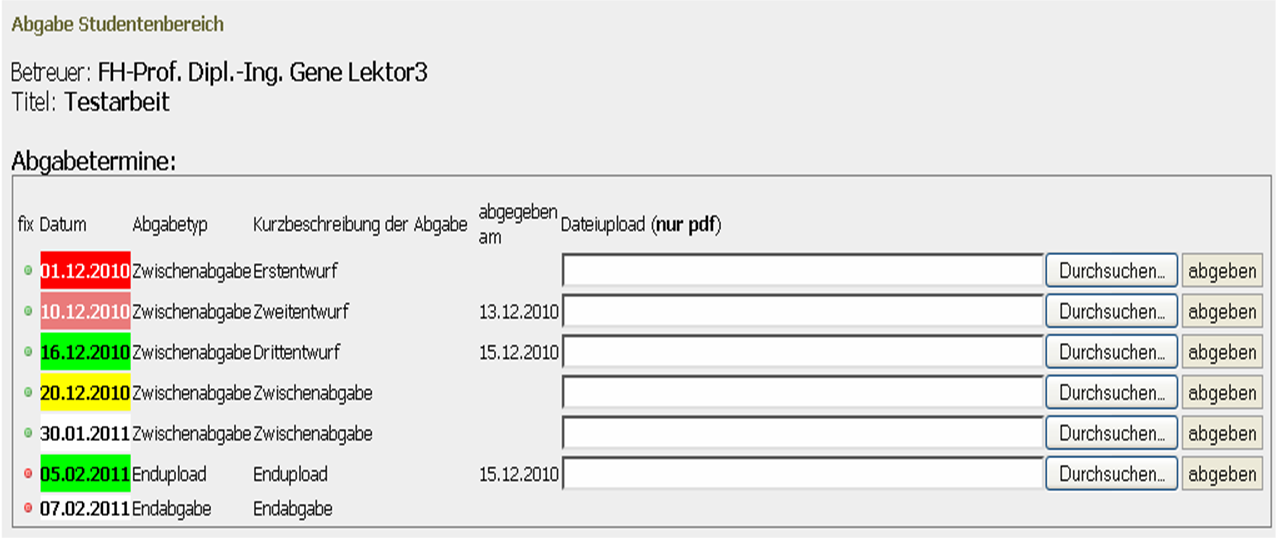
\includegraphics[width=1.0\textwidth]{abgabetool_termine_student}
	\caption{Deadline Overview}
	\label{abgabetool_termine_student}
\end {figure}

\subsection{Deadlines and File Upload}

\begin{itemize}
	\item The different deadlines (first draft, interim submission, final submission,...) are displayed here in rows. 
	\item The color code indicates the deadline status (see chapter \ref{farbcode}).
	\item Click on \textit{Search} in the relevant deadline to browse your hard drive for the desired file. Next, click on \textit{Submit} to send the file. Your supervisor will automatically be notified of your submission by email. If you upload a file again, the existing file will be overwritten.	
	\item The administrative assistant can assign fixed deadlines which can be recognized by the red bullet in the column \textit{fixed}. If a fixed deadline has expired, you will no longer be able submit any files for this deadline. If something should still need to be uploaded, you must ask the administrative assistant to correct the deadline.
	
	\info{Files can currently only be uploaded in PDF format.}
\end{itemize}

\subsection{Color Code}
\label{farbcode}

\begin{itemize}
	\item White:	"'Normal"' deadline
	\item Yellow:	Deadline within the next 12 days
	\item Red:	Deadline expired
	\item Green:	Submission has been made
	\item Light Red: Submitted after the deadline 
\end{itemize}

\subsection{Additional Data for the Final Submission}
Once the \textit{final submission} has finished uploading, a form will appear (see Fig. \ref{abgabetool_zusatzdaten_student}) that will prompt you to enter additional data for the publication database. Your supervisor will also check this data to ensure it is complete.

\begin {figure}
	\centering
	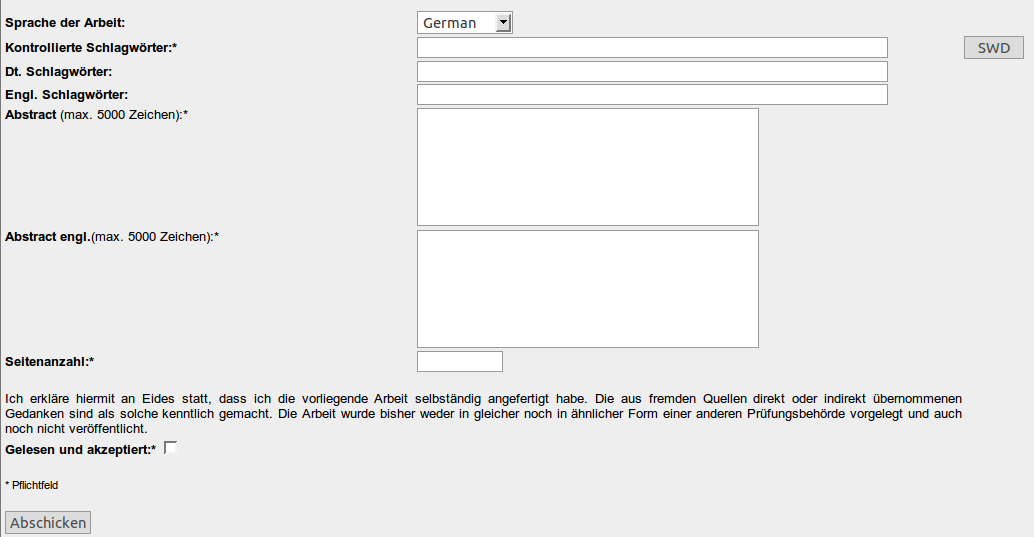
\includegraphics[width=1.0\textwidth]{abgabetool_zusatzdaten_student}
	\caption{Additional Data after the Final Submission}
	\label{abgabetool_zusatzdaten_student}
\end {figure}
